% CONFIGURAÇÃO VISUAL — os textos ficam em ../main.tex.
\usepackage[utf8]{inputenc}
\usepackage[T1]{fontenc}
\usepackage{lmodern}
\usepackage{tikz}
\usepackage{anyfontsize}
\usetikzlibrary{arrows.meta,positioning,calc}
\usetheme{default}
\definecolor{Ink}{RGB}{54,39,34}
\definecolor{Amber}{RGB}{172,76,22}
\definecolor{Honey}{RGB}{227,167,64}
\definecolor{Cream}{RGB}{249,245,236}
\definecolor{Muted}{RGB}{114,96,82}
\setbeamercolor{normal text}{fg=Ink,bg=white}
\setbeamercolor{structure}{fg=Amber}
\setbeamercolor{frametitle}{fg=Ink,bg=Cream}
\setbeamercolor{block title}{fg=Amber,bg=Cream}
\setbeamercolor{block body}{fg=Ink,bg=Cream}
\setbeamerfont{frametitle}{size=\Large,series=\bfseries}
\setbeamerfont{framesubtitle}{size=\small}
\setbeamersize{text margin left=0.8cm,text margin right=0.8cm}
\setbeamertemplate{navigation symbols}{}
\setbeamertemplate{itemize item}{\color{Amber}\small\textbullet}
\setbeamertemplate{frametitle}{%
  \nointerlineskip
  \begin{beamercolorbox}[wd=\paperwidth,sep=0.17cm,leftskip=0.63cm,rightskip=0.63cm]{frametitle}
    {\usebeamerfont{frametitle}\strut\insertframetitle\strut\par}
    {\usebeamerfont{framesubtitle}\color{Muted}\strut\insertframesubtitle\strut\par}
  \end{beamercolorbox}%
}
\setbeamertemplate{footline}{%
  \hbox{\hspace{0.8cm}\color{Honey}\rule{\dimexpr\paperwidth-1.6cm\relax}{0.5pt}}%
  \vskip0.08cm
  \hbox to\paperwidth{\hspace{0.8cm}%
    {\color{Amber}\fontsize{7.5}{9}\selectfont VINHO LARANJA}%
    \hspace{0.25cm}{\color{Muted}\fontsize{7.5}{9}\selectfont Processo e identidade sensorial}%
    \hfill{\color{Ink}\fontsize{8}{9}\selectfont\insertframenumber\,/\,\inserttotalframenumber}%
    \hspace{0.8cm}}
  \vskip0.15cm
}
\newcommand{\kicker}[1]{{\color{Amber}\fontsize{9}{11}\selectfont\bfseries #1}\par\vspace{0.12cm}}
\newcommand{\bodytext}[1]{{\fontsize{12}{16}\selectfont #1\par}}
\newcommand{\smalltext}[1]{{\fontsize{10.5}{14}\selectfont #1\par}}
\newcommand{\source}[1]{\par\vspace{0.18cm}{\color{Muted}\fontsize{7.5}{9}\selectfont Fontes: #1.\par}}
\newcommand{\callout}[1]{%
  \par\vspace{0.18cm}
  \begin{beamercolorbox}[wd=\linewidth,sep=0.19cm]{block body}
    \fontsize{11}{14}\selectfont #1
  \end{beamercolorbox}}
\newcommand{\card}[3]{%
  \begin{beamercolorbox}[wd=\linewidth,sep=0.24cm]{block body}
    {\color{Amber}\fontsize{9}{11}\selectfont\bfseries #1}\par\vspace{0.17cm}
    {\fontsize{16}{19}\selectfont\bfseries #2}\par\vspace{0.17cm}
    {\fontsize{11}{15}\selectfont #3}\par
  \end{beamercolorbox}}
% Taça esquemática em vetor.
\newcommand{\wineglass}{%
  
\begin{tikzpicture}[x=1cm,y=1cm,scale=1.05]
    \fill[Honey] (-0.99,1.60) .. controls (-0.83,0.75) and (-0.48,0.30) .. (0,0.30)
      .. controls (0.48,0.30) and (0.83,0.75) .. (0.99,1.60) -- cycle;
    \draw[white,line width=1.1pt] (-1.15,2.75) -- (-1.05,1.90)
      .. controls (-0.95,0.80) and (-0.50,0.25) .. (0,0.25)
      .. controls (0.50,0.25) and (0.95,0.80) .. (1.05,1.90) -- (1.15,2.75) -- cycle;
    \draw[white,line width=1.1pt] (0,0.25) -- (0,-1.1);
    \draw[white,line width=1.1pt] (-0.72,-1.1) -- (0.72,-1.1);
    \draw[white,opacity=0.65,line width=1.2pt] (-0.83,2.40) -- (-0.76,1.94);
  \end{tikzpicture}}
% Qvevri esquemático: vaso de argila em contato com o solo.
\newcommand{\qvevri}{%
  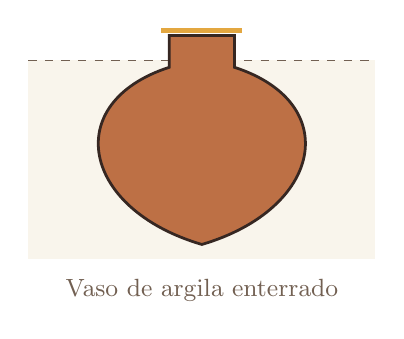
\begin{tikzpicture}[scale=0.90]
    \fill[Cream] (-2.45,-2.2) rectangle (2.45,0.6);
    \draw[Muted,dashed] (-2.45,0.6) -- (2.45,0.6);
    \fill[Amber!80] (-0.46,0.95) -- (-0.46,0.5)
      .. controls (-2.0,-0.0) and (-1.70,-1.50) .. (0,-2.0)
      .. controls (1.70,-1.50) and (2.0,-0.0) .. (0.46,0.5) -- (0.46,0.95) -- cycle;
    \draw[Ink,line width=1pt] (-0.46,0.95) -- (-0.46,0.5)
      .. controls (-2.0,-0.0) and (-1.70,-1.50) .. (0,-2.0)
      .. controls (1.70,-1.50) and (2.0,-0.0) .. (0.46,0.5) -- (0.46,0.95) -- cycle;
    \draw[Honey,line width=2pt] (-0.57,1.02) -- (0.57,1.02);
    \node[font=\small,text=Muted] at (0,-2.65) {Vaso de argila enterrado};
  \end{tikzpicture}}
